% F06: Section 5.3: Physical Demonstrations and Failure Analysis. Read figures/FIGURE_GUIDE.md before reuse.
\begin{figure}[tbp]
  \centering
  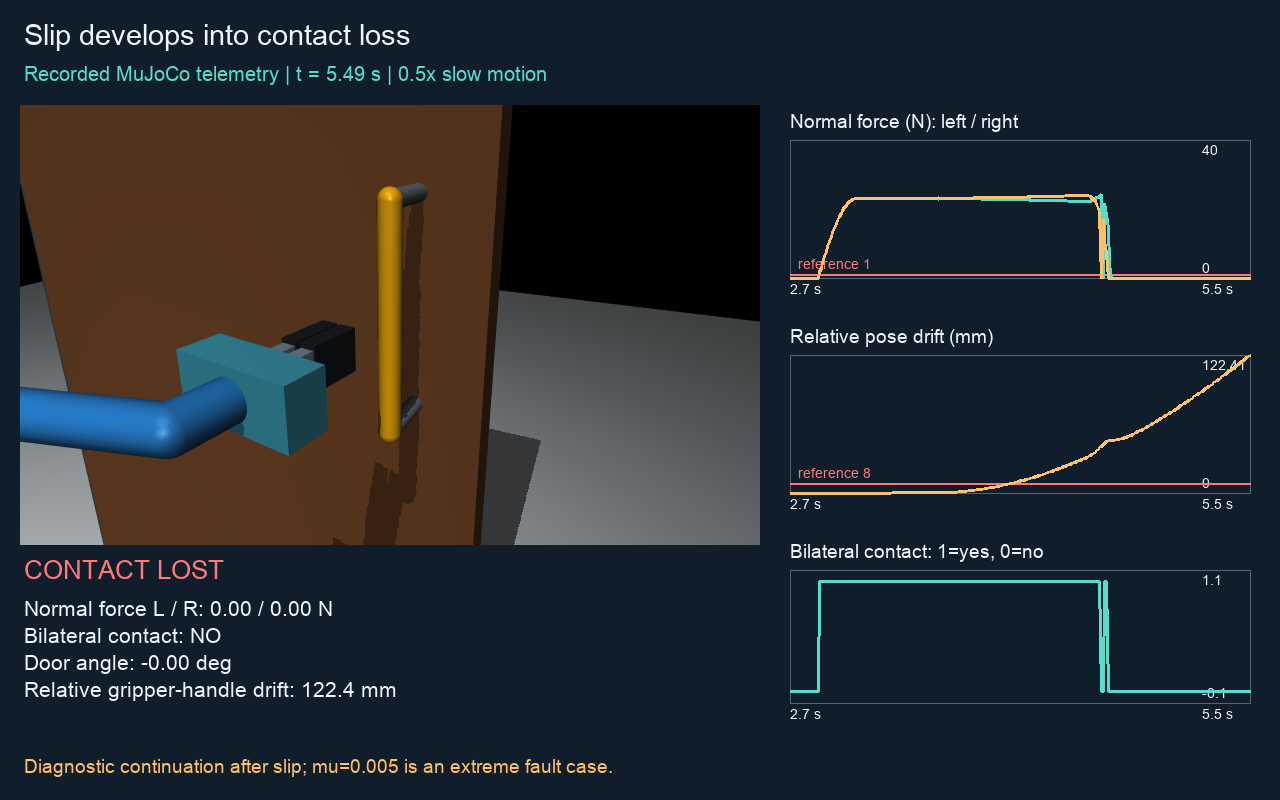
\includegraphics[width=1.0\linewidth]{figures/failures/F06_slip_contact_loss.png}
  \caption{Diagnostic low-friction replay ($\mu=0.005$). A slip alarm occurs at approximately 3.77 s and persistent contact loss at 4.73 s. At the displayed 5.49 s sample, both contact forces are zero and the relative separation is about 122.4 mm. Execution deliberately continues after the slip alarm; separation after release is not ongoing surface slip.}
  \label{fig:slip_contact_loss}
\end{figure}
